\documentclass{article}
\usepackage[utf8]{inputenc}
\usepackage{geometry}
\usepackage{amsmath}
\usepackage{url}
\usepackage[utopia]{mathdesign}
\usepackage{lipsum}  
\usepackage{lmodern}
\usepackage{listings}
\usepackage{tikz}
\usetikzlibrary{arrows.meta, positioning}

 \geometry{
 a4paper,
 total={170mm,257mm},
 left=20mm,
 top=20mm,
 }
 \usepackage{graphicx}
 \usepackage{titling}

 \title{Report \#8}
\author{GU JUN}
 
 \usepackage{fancyhdr}
\fancypagestyle{plain}{%  the preset of fancyhdr 
    \fancyhf{} % clear all header and footer fields
%    \fancyfoot[R]{\includegraphics[width=5cm]{}}
    \fancyfoot[L]{\today}
    \fancyhead[L]{Analytical Mechanics 80848\#8}
    \fancyhead[R]{HIRAI SHINCHI}
}
\makeatletter
\renewcommand{\maketitle}{%
  \newpage
  \null
  \vskip 1em%
  \begin{center}%
  \let \footnote \thanks
    {\LARGE \@title \par}%
    \vskip 1em%
    %{\large \@date}%
  \end{center}%
  \par
  \vskip 1em}
\makeatother


\begin{document}

\maketitle

\noindent\begin{tabular}{@{}ll}
    Student & \theauthor\\
    ID number & 6132230056 \\
\end{tabular}
\section*{Deformation simulation of a viscoelastic object}
Simulate the deformation of a rectangular viscoelastic object shown in the figure. 
The bottom surface is fixed to the ground. 
A pair of forces with the same magnitude $f$ are applied to the both sides for a while, then the forces are released. 
Action lines of the forces do not coincide. 
Use appropriate values of geometrical and physical parameters of the object.
\begin{center}
  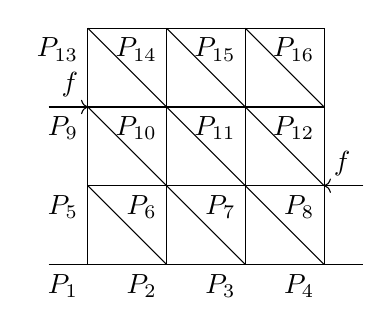
\begin{tikzpicture}
      % Define points
      \coordinate (P1) at (0, 0); 
      \coordinate (P2) at (1, 0);
      \coordinate (P3) at (2, 0);
      \coordinate (P4) at (3, 0);
      \coordinate (P5) at (0, 1);
      \coordinate (P6) at (1, 1);
      \coordinate (P7) at (2, 1);
      \coordinate (P8) at (3, 1);
      \coordinate (P9) at (0, 2);
      \coordinate (P10) at (1, 2);
      \coordinate (P11) at (2, 2);
      \coordinate (P12) at (3, 2);
      \coordinate (P13) at (0, 3);
      \coordinate (P14) at (1, 3);
      \coordinate (P15) at (2, 3);
      \coordinate (P16) at (3, 3);
  
      % Draw axes
      \draw[->] (-0.5, 2) -- (0, 2) node[above left] {$f$};
      \draw[->] (3.5, 1) -- (3, 1) node[above right] {$f$};
      \draw (-0.5, 0) -- (3.5, 0);
  
      % Draw main structure
      \draw (P1) -- (P4) -- (P16) -- (P13) -- cycle; % Outer shape
      \draw (P5) -- (P8);
      \draw (P9) -- (P12);
      \draw (P2) -- (P14);
      \draw (P3) -- (P15);
      \draw (P5) -- (P2);
      \draw (P6) -- (P3);
      \draw (P7) -- (P4);
      \draw (P9) -- (P6);
      \draw (P10) -- (P7);
      \draw (P11) -- (P8);
      \draw (P13) -- (P10);
      \draw (P14) -- (P11);
      \draw (P15) -- (P12);
  
      % Label points
      \node[below left] at (P1) {$P_1$};
      \node[below left] at (P2) {$P_2$};
      \node[below left] at (P3) {$P_3$};
      \node[below left] at (P4) {$P_4$};
      \node[below left] at (P5) {$P_5$};
      \node[below left] at (P6) {$P_6$};
      \node[below left] at (P7) {$P_7$};
      \node[below left] at (P8) {$P_8$};
      \node[below left] at (P9) {$P_9$};
      \node[below left] at (P10) {$P_{10}$};
      \node[below left] at (P11) {$P_{11}$};
      \node[below left] at (P12) {$P_{12}$};
      \node[below left] at (P13) {$P_{13}$};
      \node[below left] at (P14) {$P_{14}$};
      \node[below left] at (P15) {$P_{15}$};
      \node[below left] at (P16) {$P_{16}$};
  \end{tikzpicture}
  \end{center}
  
\section*{Preset}
We first define the rectangular object as a 2D grid with $4 \times 4$ points, and the height and the width of the object are $3$ and $3$ respectively.
The thickness of the object is $1$. The material properties of the viscoelastic object are defined as follows: Young's modulus $E = 1.0 \times 10^6$ Pa, damping coefficient $c = 0.04 \times 10^3$ Ns/m, Poisson's ratio $\nu = 0.48$, and density $\rho = 0.020$ kg/m$^3$.\\
According to the problem, we need to define the following constraints:
\begin{itemize}
    \item The bottom surface is fixed to the ground.
    \item A pair of forces with the same magnitude $f$ are applied to the both sides for a while, then the forces are released.
\end{itemize}

According to this two constraints, we can define the following constraint matrix $A$:
\[
A = 
  \begin{bmatrix}
  1 & 0 & 0 & 0 & 0 & 0 & 0 & 0 \\
  0 & 1 & 0 & 0 & 0 & 0 & 0 & 0 \\
  0 & 0 & 1 & 0 & 0 & 0 & 0 & 0 \\
  0 & 0 & 0 & 1 & 0 & 0 & 0 & 0 \\
  0 & 0 & 0 & 0 & 1 & 0 & 0 & 0 \\
  0 & 0 & 0 & 0 & 0 & 1 & 0 & 0 \\
  0 & 0 & 0 & 0 & 0 & 0 & 1 & 0 \\
   0 & 0 & 0 & 0 & 0 & 0 & 0 & 1 \\
   \multicolumn{8}{c}{\vdots} \\
   0 & 0 & 0 & 0 & 0 & 0 & 0 & 0 \\
  \end{bmatrix}
\]

And the external force matrix $F$:
\[
F = 
  \begin{bmatrix}
  0, 
  \dots, 
  $ f$,  
  $-f$,
  \dots,
  0 
  \end{bmatrix}^\top
\]
Here $f$ is the magnitude of the force applied to the object, I will set $f = 0.8 \times 10^6$ N.\\
The time length with the force applied is $0.1$ s, and the time length with the force released is $0.9$ s. The total time length of the simulation is $1$ s.\\
With the above parameters, we can simulate the deformation of the viscoelastic object.\\
\newpage
\section*{Simulation Results}
\begin{figure}[htbp]
  \centering
  \begin{tabular}{ccccccc}
    \includegraphics[width=0.2\textwidth]{assets/deform_0000.png} & 
    \includegraphics[width=0.2\textwidth]{assets/deform_0050.png} & 
    \includegraphics[width=0.2\textwidth]{assets/deform_0100.png} &
    \includegraphics[width=0.2\textwidth]{assets/deform_0150.png} & 
    \includegraphics[width=0.2\textwidth]{assets/deform_0200.png} & 
    \includegraphics[width=0.2\textwidth]{assets/deform_0250.png} &
    \includegraphics[width=0.2\textwidth]{assets/deform_0300.png} \\ 
    \includegraphics[width=0.2\textwidth]{assets/deform_0350.png} & 
    \includegraphics[width=0.2\textwidth]{assets/deform_0400.png} &
    \includegraphics[width=0.2\textwidth]{assets/deform_0450.png} & 
    \includegraphics[width=0.2\textwidth]{assets/deform_0500.png} & 
    \includegraphics[width=0.2\textwidth]{assets/deform_0550.png} &
    \includegraphics[width=0.2\textwidth]{assets/deform_0600.png} & 
    \includegraphics[width=0.2\textwidth]{assets/deform_0650.png} \\ 
    \includegraphics[width=0.2\textwidth]{assets/deform_0700.png} &
    \includegraphics[width=0.2\textwidth]{assets/deform_0750.png} & 
    \includegraphics[width=0.2\textwidth]{assets/deform_0800.png} & 
    \includegraphics[width=0.2\textwidth]{assets/deform_0850.png} &
    \includegraphics[width=0.2\textwidth]{assets/deform_0900.png} & 
    \includegraphics[width=0.2\textwidth]{assets/deform_0950.png} & 
    \includegraphics[width=0.2\textwidth]{assets/deform_1000.png} \\
  \end{tabular}
  \caption{Deformation simulation results at different time steps}
  \label{fig:deformation}
\end{figure}
\section*{Appendix}
\scriptsize
\begin{lstlisting}{language=MATLAB}
  m = 4; n = 4;
thickness = 1;
[ points, triangles ] = rectangular_object( m, n, 3, 3 );

% E = 0.1 MPa; c = 0.004 kPa s; rho = 0.020 g/cm^3
Young = 1.0*1e+6; c = 0.04*1e+3; nu = 0.48; density = 0.020;

[ lambda, mu ] = Lame_constants( Young, nu );
[lambda_vis, mu_vis] = Lame_constants(c, nu);

npoints = size(points,2);
ntriangles = size(triangles,1);
elastic = Body(npoints, points, ntriangles, triangles, thickness);
elastic = elastic.mechanical_parameters(density, lambda, mu);
elastic = elastic.viscous_parameters(lambda_vis, mu_vis);
elastic = elastic.calculate_stiffness_matrix;
elastic = elastic.calculate_damping_matrix;
elastic = elastic.calculate_inertia_matrix;

alpha = 1e+6;
A = elastic.constraint_matrix([1,2,3,4]);
b0 = zeros(2*4,1);
b1 = zeros(2*4,1);

tp = 0.1;
tf = 0.9;
fpush = -0.8*1e+6;
        
% external force
interval = [0,tp];
qinit = zeros(4*npoints,1);
external = zeros(2*npoints,1);
external(8) = fpush;
external(9) = -fpush;
beam_bending_external_force = @(t,q) beam_bending_external_force_param_Cauchy_strain(t,q, elastic, A,b0,b1, external, alpha);
[time_push, q_push] = ode15s(beam_bending_external_force, interval, qinit);
%[time_push, q_push] = ode45(beam_bending_external_force, interval, qinit);

\end{lstlisting}

\end{document}
